% --- SECTION 3 : L'ORDINATEUR DE PLONGÉE ---
\section{L'ordinateur de plongée}

\begin{frame}{Transition : De la Table à l'Ordinateur}
    \footnotesize
    \begin{columns}[c]
        \begin{column}{0.5\textwidth}
            \centering
            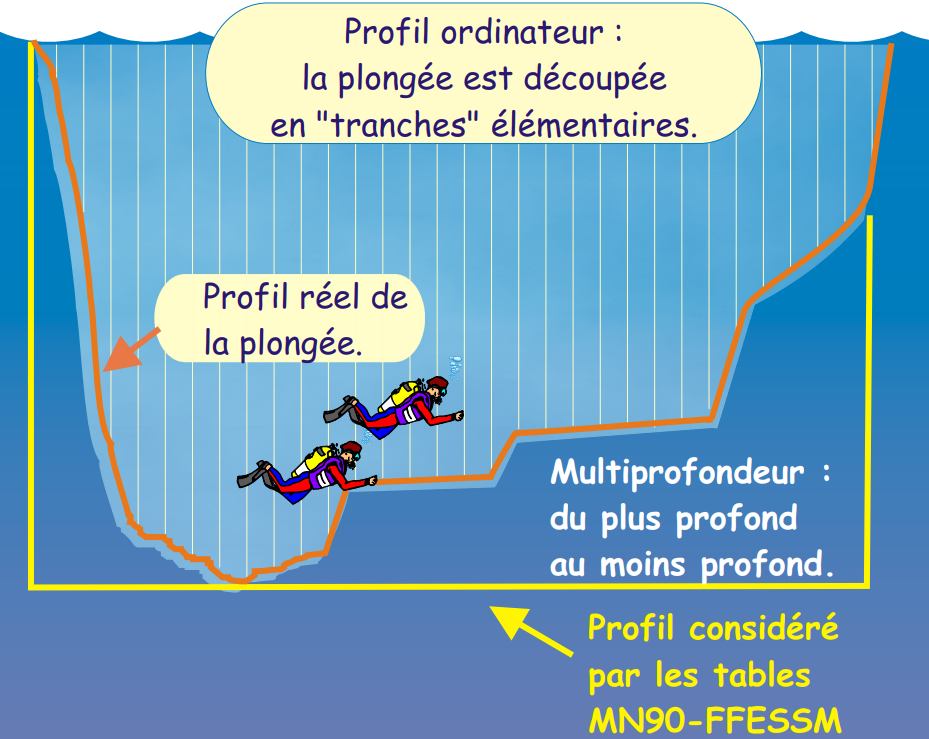
\includegraphics[width=\columnwidth]{images/table_vs_ordinateur}
        \end{column}

        \begin{column}{0.5\textwidth}
            \textbf{La Logique des Tables :}
            \begin{itemize}
                \setlength\itemsep{0em}
                \item Elles considèrent un \textbf{profil carré}.
                \item Hypothèse : Tout le temps de plongée est passé à la profondeur \textbf{maximale}.
                \item \textit{Conséquence :} Pénalisant pour les plongées multi-niveaux.
            \end{itemize}

            \textbf{La Logique de l'Ordinateur :}
            \begin{itemize}
                \setlength\itemsep{0em}
                \item Il suit le \textbf{profil réel} (ligne orange).
                \item Calcul dynamique : La plongée est découpée en "tranches" élémentaires pour ajuster la saturation en temps réel.
            \end{itemize}
            \vspace{-0.1cm}
            \begin{exampleblock}{Le Bénéfice pour le Plongeur N3}
                L'ordinateur optimise le temps de plongée sans palier (courbe de sécurité) en prenant en compte la remontée progressive.
            \end{exampleblock}
        \end{column}
    \end{columns}
\end{frame}

\begin{frame}{Principe et fonctionnement}
    \begin{center}
    \resizebox{!}{0.8\textheight}
    {
        \begin{tikzpicture}[
    node distance=1.5cm and 1.2cm,
    box/.style={
        rectangle, 
        draw=blue!70!black, 
        fill=blue!10, 
        very thick, 
        text centered, 
        minimum width=2.5cm, 
        minimum height=1cm,
        font=\sffamily\small\bfseries
    },
    main/.style={
        box, 
        fill=blue!30, 
        minimum width=4cm, 
        minimum height=2cm,
        text width=3.5cm
    },
    arrow/.style={
        -Stealth, 
        thick, 
        draw=gray!80
    }
]

% --- Noeuds (Positions) ---

% Centre
\node[main] (cpu) {MICROPROCESSEUR (Calculateur)};

% Entrées Gauche
\node[box, left=of cpu] (gas) {Réglage Gaz ($\% O_2$)};
\node[box, above=of gas] (temp_sens) {Capteur de Température};
\node[box, below=of gas, xshift=-1cm] (user) {Boutons (Interface Utilisateur)};

% Capteurs Haut
\node[box, above=of cpu] (press) {Capteur de Pression};
\node[box, right=of press] (depth) {Suivi Profondeur/Temps};

% Calcul et Mémoire
\node[box, right=of cpu, text width=2.8cm] (algo) {Modèle de Décompression (Bühlmann, RGBM...)};
\node[box, below=of cpu, yshift=-1cm] (log) {Mémoire (Carnet de plongée)};

% Sortie
\node[box, below=of algo, xshift=1.5cm, fill=blue!50, minimum width=4cm, minimum height=1.5cm, text width=4.5cm] (screen) 
    {ÉCRAN D'AFFICHAGE \mdseries \footnotesize (Prof., DTR, No-Deco, Temps, Temp., Gaz)};

% --- Flèches (Connexions) ---

\draw[arrow] (press) -- (cpu);
\draw[arrow] (press) -- (depth);
\draw[arrow] (temp_sens) -- (cpu);
\draw[arrow] (gas) -- (cpu);
\draw[arrow] (user) -- (cpu);
\draw[arrow] (cpu) -- (algo);
\draw[arrow] (algo) -- (screen);
\draw[arrow] (log) -- (screen.west);
\draw[arrow] (depth) -- (algo);
\draw[arrow] (cpu) |- ($(screen.north west)!0.25!(screen.south west)$);
\draw[arrow] ($(algo.south west)!0.25!(algo.south east)$) -- ++(0,-0.5) -| ($(cpu.south west)!0.75!(cpu.south east)$);

\path ($(cpu.south west)!0.25!(cpu.south east)$) coordinate (START);
\draw[arrow] (START) -- (START |- log.north);
\end{tikzpicture}  
    }
    \end{center}
\end{frame}

\begin{frame}{Informations affichées}
    \begin{columns}
        \begin{column}{0.6\textwidth}
            \textbf{Pendant la plongée :}
            \begin{itemize}
                \item Profondeur actuelle et maximale[cite: 13, 379].
                \item Temps d'immersion[cite: 12, 380].
                \item \textbf{No Deco :} Temps restant avant palier[cite: 20, 380].
                \item Vitesse de remontée[cite: 13, 380].
            \end{itemize}
            \textbf{En zone de palier :}
            \begin{itemize}
                \item Profondeur du palier le plus bas[cite: 23].
                \item \textbf{DTR :} Durée Totale de Remontée (inclut la montée et tous les paliers)[cite: 22, 1723].
            \end{itemize}
        \end{column}
        \begin{column}{0.4\textwidth}
            \centering
            %\includegraphics[width=\textwidth]{ecran_ordi.png}
            \textit{Note : Toujours lire la notice de son propre modèle[cite: 17, 35].}
        \end{column}
    \end{columns}
\end{frame}

\begin{frame}{Sécurité et procédures en palanquée}
    \begin{itemize}
        \item \textbf{Gestion de la palanquée :} En cas d'ordinateurs différents, on suit toujours le plus \textbf{pénalisant} (celui qui affiche le plus de paliers)[cite: 25, 384].
        \item \textbf{Panne d'ordinateur :} 
        \begin{itemize}
            \item Interruption immédiate de la plongée[cite: 26].
            \item Remontée lente et respect des paliers du binôme (ou majoration de sécurité)[cite: 26, 41].
            \item \textbf{Pas de ré-immersion avant 24h}[cite: 26].
        \end{itemize}
        \item \textbf{Alarme :} Respecter impérativement les alertes de vitesse de remontée (risque d'ADD)[cite: 19, 380].
    \end{itemize}
\end{frame}
